\item \begin{theorem}{(441)} 原始pipeline設計:\begin{itemize}
        \item \code{beq}在$MEM$決定是否要跳。
        \item \code{RegDst}在$EX$。
    \end{itemize}
    \begin{figure}[H]
        \centering
        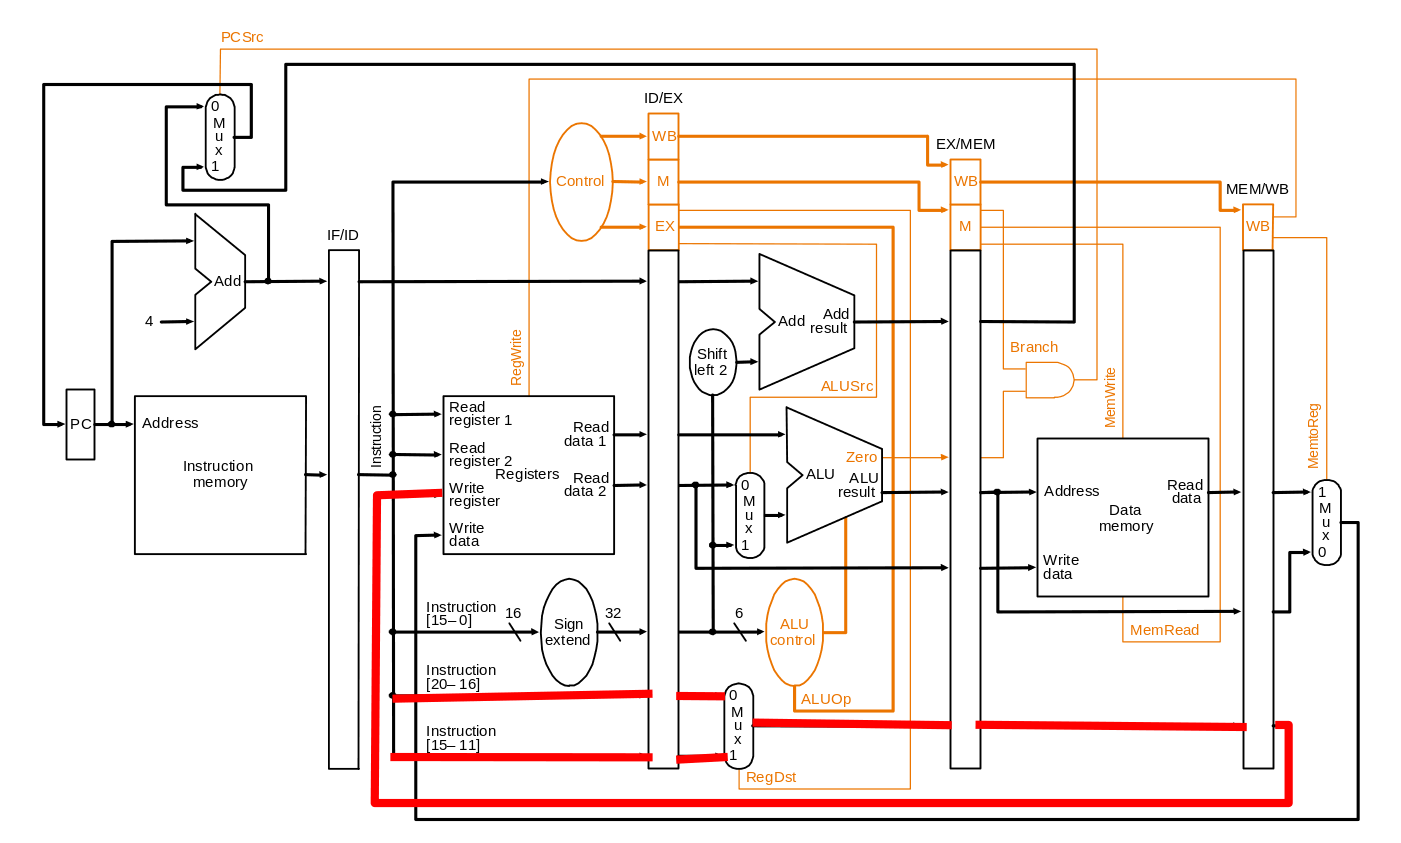
\includegraphics[scale=0.3]{img/pipeline-org.png}
        \caption{Original pipeline.}
        \label{img:pipeline-org}
    \end{figure}
\end{theorem}

\item \begin{theorem}{(450, 455, 457, 458)} Data hazards:\begin{itemize}
        \item Forwarding:Combinational units,放在$EX$因為ALU。
        \begin{lstlisting}[caption={EX hazard.}, captionpos=b, mathescape=true, language={[x86masm]Assembler}, autogobble=true]
            if (EX/MEM.RegWrite $\land$ (EX/MEM.Rd $\neq 0$) $\land$ 
                (EX/MEM.Rd $=$ ID/EX.Rs/Rt))
                ForwardA/B = $10$
        \end{lstlisting}
        \begin{lstlisting}[caption={MEM hazard.}, captionpos=b, mathescape=true, language={[x86masm]Assembler}, autogobble=true]
            if (MEM/WB.RegWrite $\land$ (MEM/WB.Rd $\neq 0$) $\land$ 
                ($\lnot$ EX_hazard) $\land$ (MEM/WB.Rd $=$ ID/EX.Rs/Rt))
                ForwardA/B = $01$
        \end{lstlisting}
        \begin{figure}[H]
            \centering
            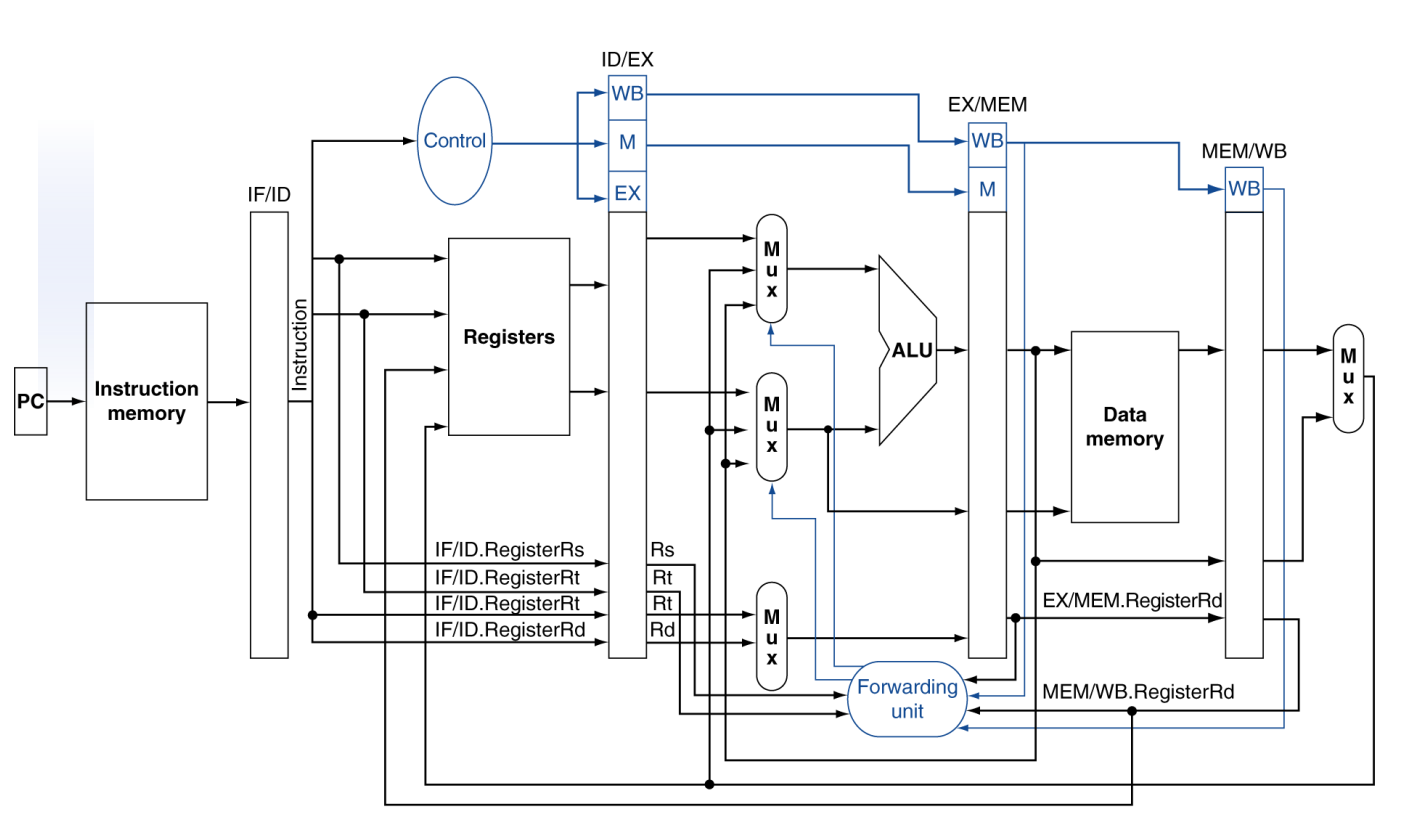
\includegraphics[scale=0.3]{img/pipeline-forward.png}
            \caption{Pipeline with forwarding.}
            \label{img:pipeline-forward}
        \end{figure}
        \item Stall:\code{}
        \begin{lstlisting}[caption={Stall.}, captionpos=b, mathescape=true, language={[x86masm]Assembler}, autogobble=true]
            if (ID/EX.MemRead $\land$ (ID/EX.Rt $=$ IF/ID.Rs/Rt))
                IF/ID.Write := $0$
                PC.Write := $0$
        \end{lstlisting}
        \begin{figure}[H]
            \centering
            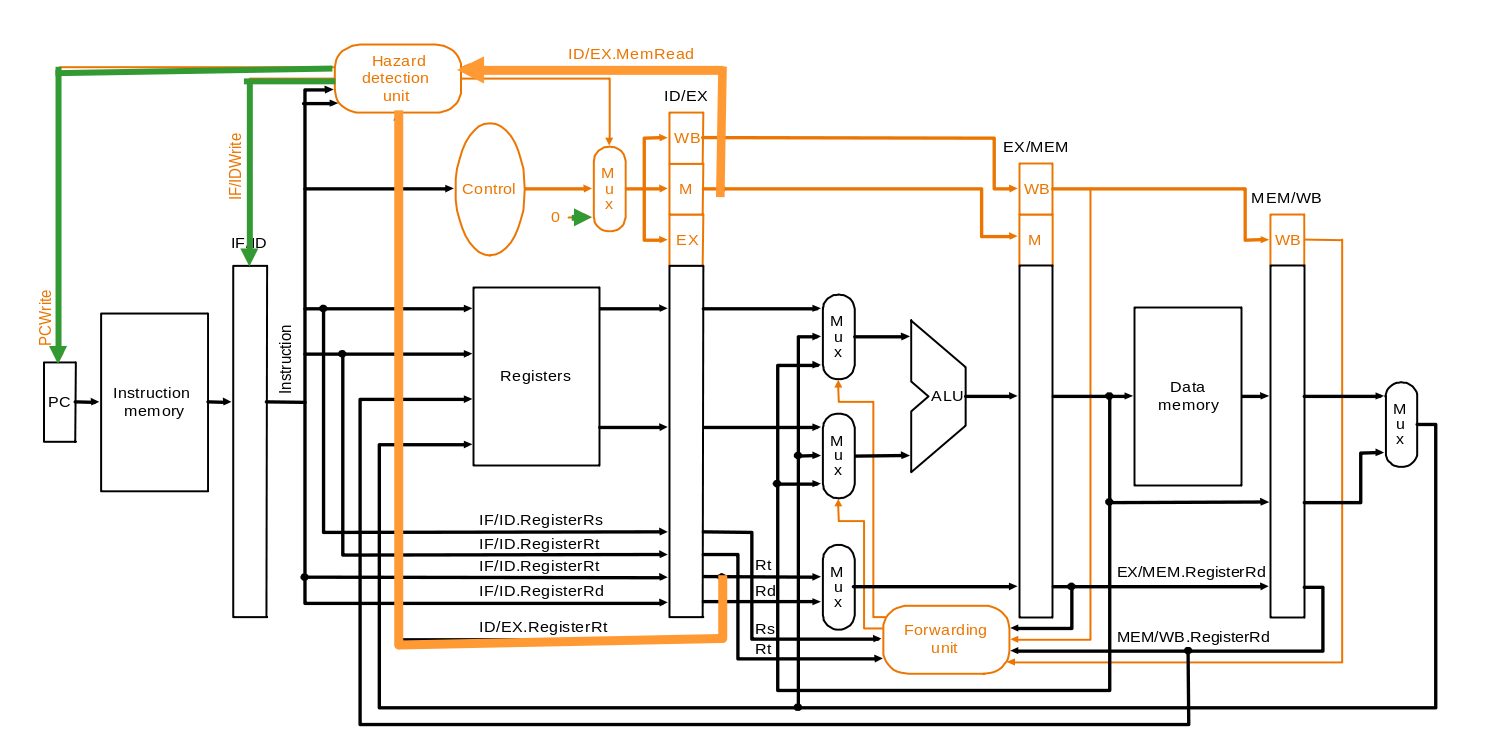
\includegraphics[scale=0.3]{img/pipeline-hazard.png}
            \caption{Pipeline with hazard detection and forwarding units.}
            \label{img:pipeline-hazard}
        \end{figure}
    \end{itemize}
\end{theorem}

\item \begin{theorem}{(478, 487, 494, 559)} Control hazards:\begin{itemize}
        \item 若分支指令與\textbf{前一個ALU指令}或\textbf{前面第二個}\code{lw}有data dependency,必須stall $1$ CC。
        \item 分支指令通過\code{xor}再\code{nor}比較是否相同。
        \begin{figure}[H]
            \centering
            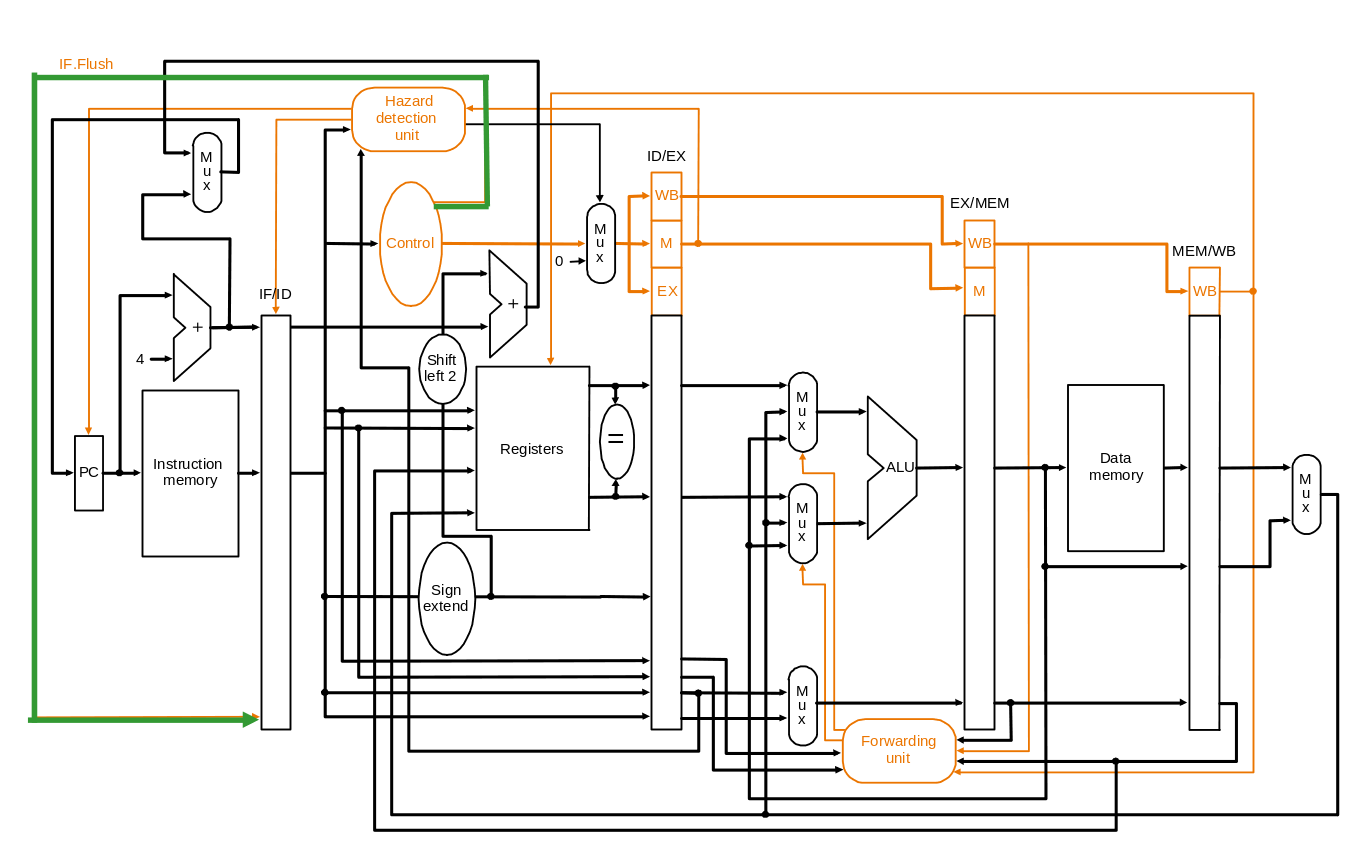
\includegraphics[scale=0.3]{img/pipeline-flush.png}
            \caption{Pipeline with hazard detection, forwarding units and flush.}
            \label{img:pipeline-flush}
        \end{figure}
        \item Delayed branch:\begin{itemize}
            \item NOT suitable for deep pipeline.
            \item From before:最佳方法,不管跳或不跳皆提升。
            \item From target:用於branch發生機率高,有跳才提升。
            \item From fall through:用於branch發生機率低,不跳才提升。
            \begin{figure}[H]
                \centering
                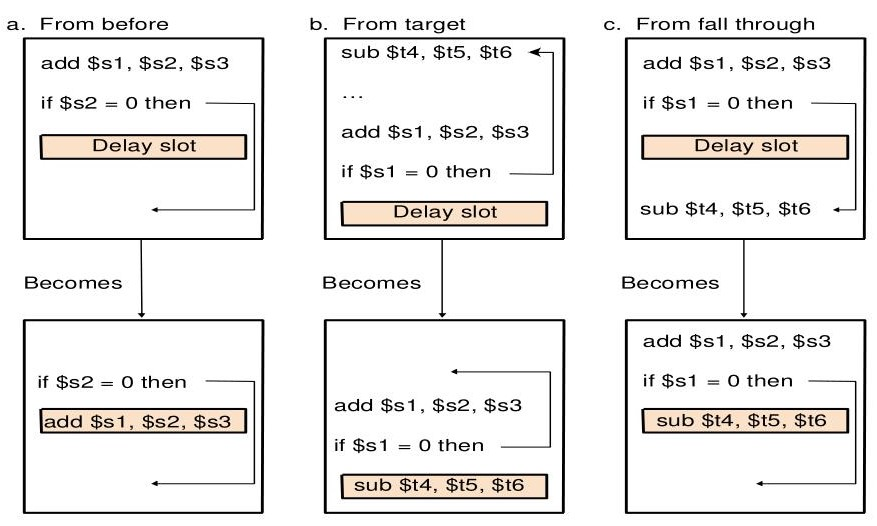
\includegraphics[scale=0.6]{img/delayed-branch.jpg}
                \caption{Example of delayed branch.}
                \label{img:delayed-branch}
            \end{figure}
        \end{itemize}
    \end{itemize}
\end{theorem}

\item \begin{theorem}{(499, 505, 511)} \quad\quad \begin{itemize}
        \item Intel IA-64 (EPIC):\begin{itemize}
            \item 支援利用compiler開發的平行度。
            \item 可以猜測,並利用if-else取代branch。
            \item Registers比MIPS多很多。
            \item Instruction group is a sequence of instructions which does \textbf{NOT} have data dependency and can be executed parallelly.
        \end{itemize}
        \item Speculation錯誤復原:\begin{itemize}
            \item 軟體提供修補程式。
            \item 硬體CPU將猜測結果暫時儲存,若正確,則將猜測結果寫回register或memory,否則flush buffer。
        \end{itemize}
        \begin{table}[H]
            \centering
            \begin{tabular}{|c|c|c|}
                \hline
                \multicolumn{3}{|c|}{Advanced pipeline} \\
                \Xhline{3\arrayrulewidth}
                Technique & Hardware & Software \\
                \Xhline{2\arrayrulewidth}
                Branch prediction & $\surd$ & $\surd$ \\
                \hline
                Speculation & $\surd$ & $\surd$ \\
                \hline
                Intel IA-64 (EPIC) & $\surd$ & $\surd$ \\
                \hline
                Register renaming & $\surd$ & $\surd$ \\
                \hline
                Prediction & & $\surd$ \\
                \hline
            \end{tabular}
        \end{table}
    \end{itemize}
\end{theorem}

\item \begin{theorem}{(515)} MIPS exception handling: \begin{itemize}
        \item 利用cause register儲存exception原因。
        \item 將造成exception的instruction memory address存在EPC ($PC + 4$)。
        \item 使用entry point switch to kernel。
        \item Exception handling routine須將$PC - 4$。
    \end{itemize}
\end{theorem}
